\documentclass{beamer}

\usepackage{xfrac}

\usetheme{default}

\title{NBICS Technologies}
\author{Alexander Aksentyev}
\institute{National Research Institute ``MEPhI''}
\date{}


\begin{document}
	\begin{frame}
		\titlepage
	\end{frame}

\section{Nano-technologies}

\begin{frame}
	\frametitle{Carbon allotropes}
	\begin{columns}
		\column{.4\textwidth}
		Allotropy is the property of some chemical elements to exist in several different geometries (known as \emph{allotropes}) in the same physical phase.
		\column{.6\textwidth}
		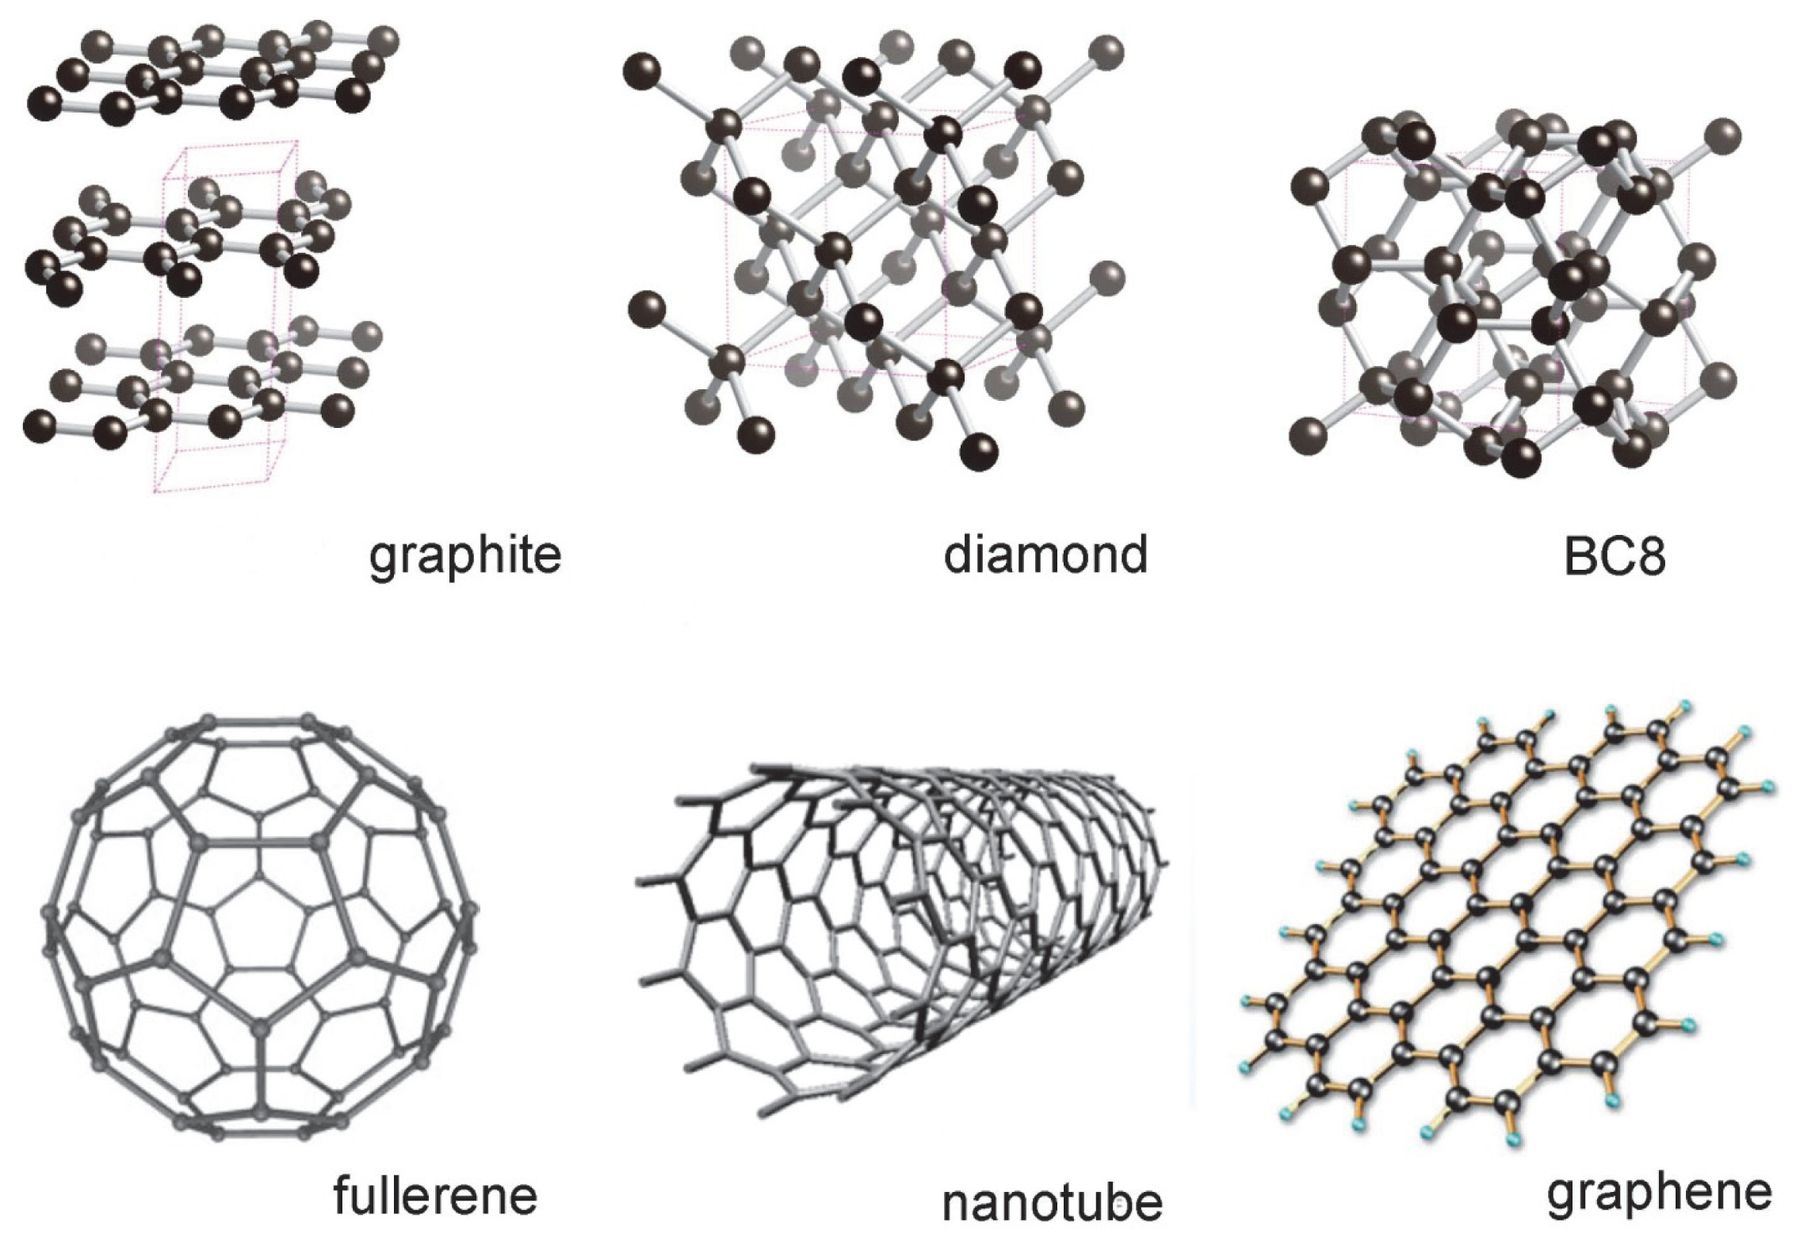
\includegraphics[scale=.45]{CarbAllotropes}
	\end{columns}
\end{frame}

\begin{frame}
	\frametitle{The nanotube}
	\begin{columns}
		\column{.45\textwidth}
		\begin{itemize}
			\item Diameter $<$ 1 nm
			\item A few nano- up to a millimeter in length
			\item Symmetry: armchair, zig-zag, chiral
			\item Single/multiple wall CNTs
			\item Compared to steel:
				\begin{itemize}
					\item 100 times more difficult to tear apart
					\item 5 times as elastic
					\item a quarter density
				\end{itemize}
			\item High thermal conductivity
			\item Metallic/semi-conductive contingent on symmetry
		\end{itemize}
		\column{.6\textwidth}
		\begin{minipage}{.5\textheight}
			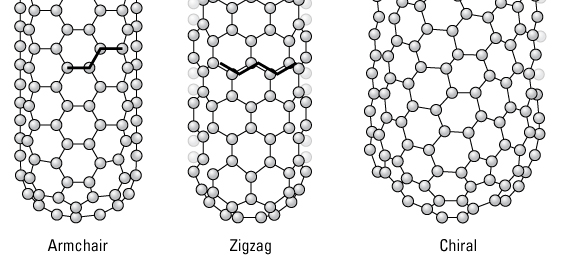
\includegraphics[scale=.65]{nanotube_orientations}
		\end{minipage}
	\begin{minipage}{.5\textheight}
		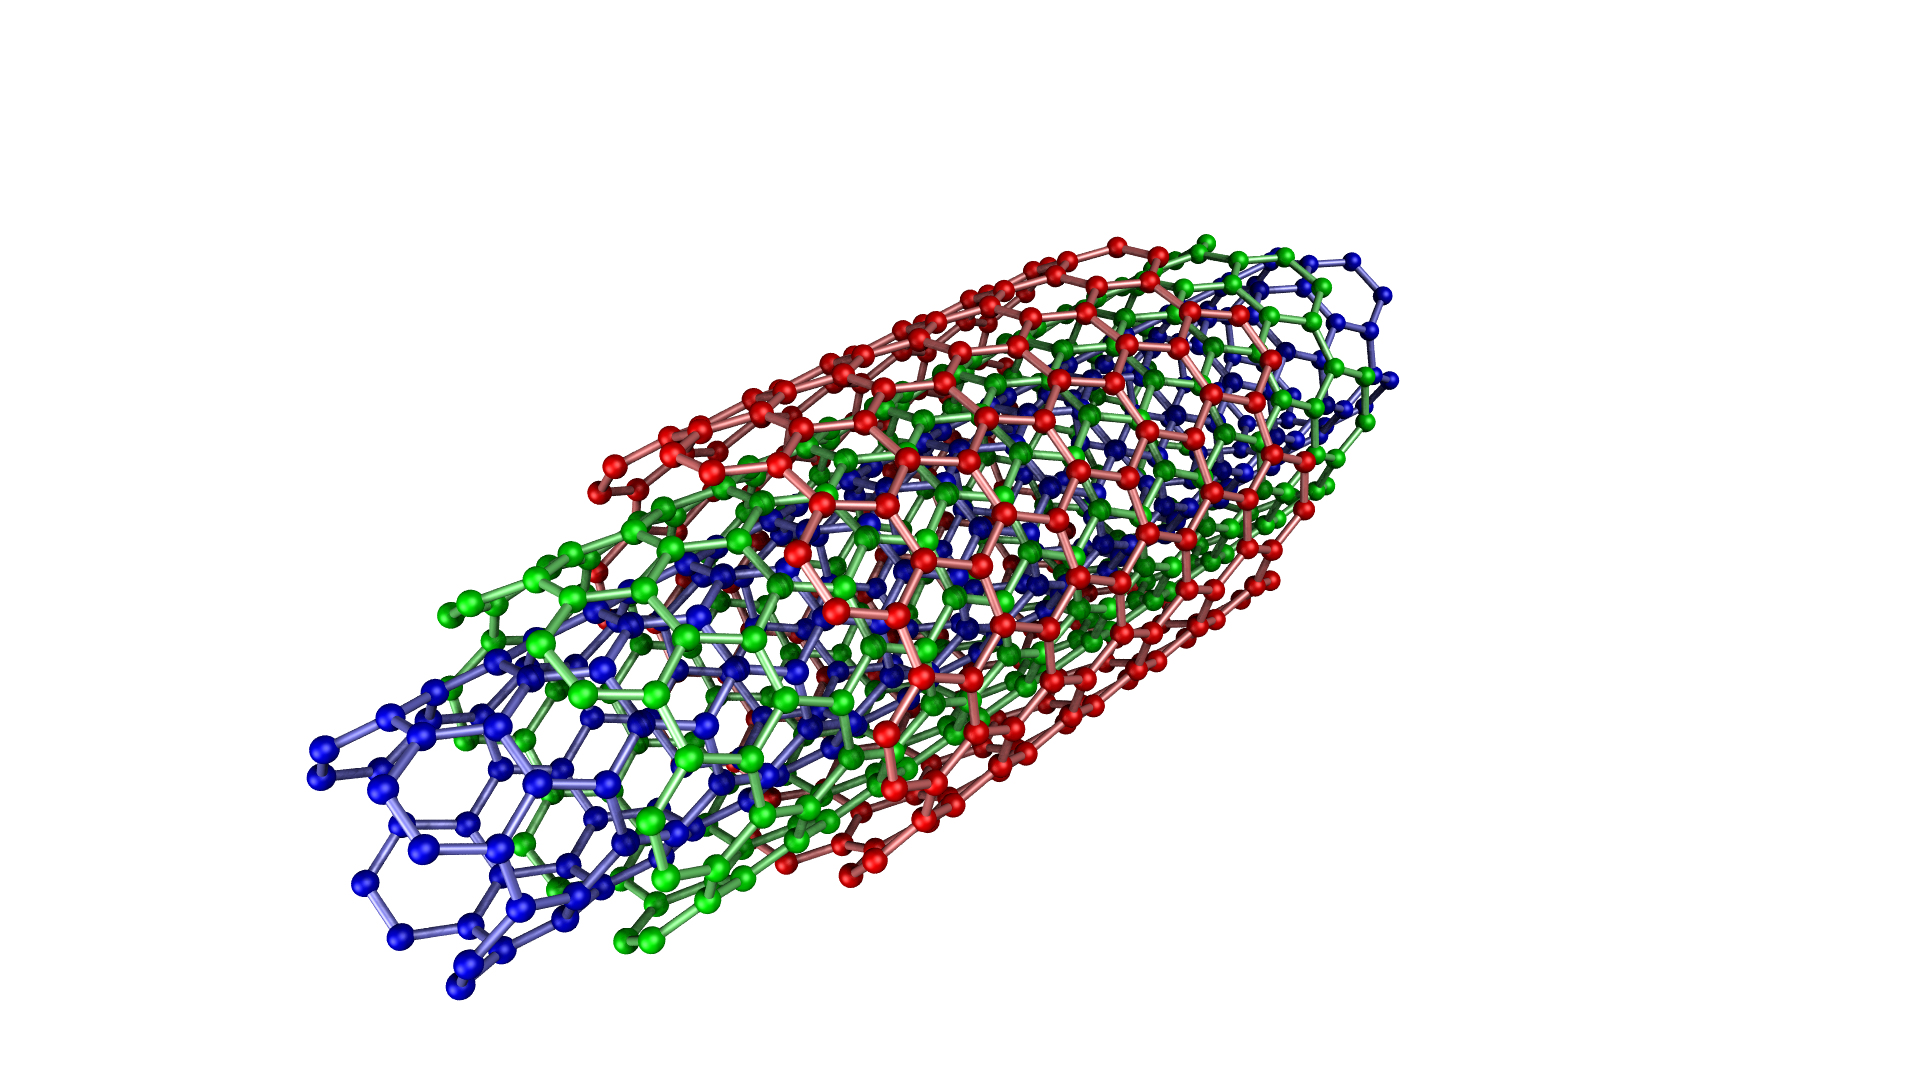
\includegraphics[scale=.1]{MWCNT}
	\end{minipage}
	\end{columns}
\end{frame}

\begin{frame}
	\frametitle{Usefulness}
	\begin{enumerate}
		\item \textbf{Energy} applications
		\begin{itemize}
			\item Pack up to 10 times more energy than Li-ion batteries
			\item Platinum substitute as a fuel cell catalyst
			\item Flexible battery geometry due to the ability to spray layers of CNTs on any surface
		\end{itemize}
		\item \textbf{Healthcare} applications
			\begin{itemize}
				\item The ability to spray thin layers + better adherence to bone than titanium's could decrease the rejection rate of dental implants by covering them in TiO$_2$ coating
				\item Natural fluorescence enables use as sensor devices, when the nanotube is attached to a binding molecule 
			\end{itemize}
		\item 
	\end{enumerate}
\end{frame}

\begin{frame}
	\frametitle{The nanobud}
\end{frame}

\section{Bio-technologies}

\section{Info-technologies}

\section{Cogno-technologies}

\section{Socio-technologies}

\end{document}